\begin{figure}[htb]
    \centering
    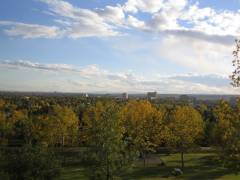
\includegraphics[width=\columnwidth]{Automatic1}
    \caption{Interface of the automatic use-case.}
    \label{fig:Automatic1}
\end{figure}

The Automatic use-case aim at executing computationally intensive applications
on the user device (e.g. browser). This scenario allow us to test if our
framework is able to act as a \emph{Distribute Computing} platform, as described
in \ref{sec:bg:crowd:auto}.


For this use-case we choose to implement an image recognition algorithm.
We used an image recognition algorithm because they are commonly used
by search engines to find images with similar features. Also these algorithms
usually have high requirements in terms of CPU load and resources usage, so they
are the perfect candidate for our purposes. The algorithm we choose to implement
was \ac{SIFT}, one of the most widely adopted for this purpose.


\subsection{\acs{SIFT} algorithm}
The \ac{SIFT} algorithm is composed of four sequential steps: Scale-space extrema
detection, Keypoint localization, Orientation assignment and Keypoint descriptor.
\begin{description}
    \item[Scale-space extrema detection:] is the stage where the interest points 
    are detected.
    \item[Keypoint localization:] is used to filter the unstable keypoints and
    keep only good keypoints.
    \item[Orientation assignment:] compute orientation and magnitude for
    each keypoint.
    \item[Keypoint descriptor:] generates the keypoints descriptors.
\end{description}

\subsubsection{Scale-space extrema detection}
In this step we generate the so called scale space representation of the image.
In order to do this we need to convolve the image $I(x,y)$ at different scales
$k\sigma$ with a varying Gaussian kernel $G(x,y,k\sigma)$ obtaining:
\[
    L(x,y,k\sigma) = G(x,y,k\sigma) \ast I(x,y)
\]
Then the difference of successive blurred images are taken
\[
    D(x,y,\sigma) = L(x,y,k_i\sigma) - L(x,y,k_j\sigma)
\]
This step produce the \ac{DoG} images, the first \emph{Keypoints} are identified
as local minima/maxima of the \ac{DoG} image across scales.



\subsubsection{Keypoint localization}
In this step the \emph{keypoints} are filtered to remove unstable points and
keep only the good ones. This step can be further subdivided into 3 stages:
\begin{itemize}
    \item \emph{Interpolation} of nearby data for accurate position.
    \item \emph{Discarding} low-contrast keypoints.
    \item \emph{Eliminating} edge responses.
\end{itemize}

\paragraph{Interpolation of nearby data for accurate position} The interpolation
is done using the quadratic Taylor expansion of the \ac{DoG} $D(x,y,\sigma)$
scale-space function, with the candidate keypoint as the origin.
This Taylor expansion is given by:
\[
    D(\mathbf{x}) = D + \frac{\partial{}D^T}{\partial{}\mathbf{x}} +
    \frac{1}{2}\cdot{}\mathbf{x}^T\cdot\frac{\partial^2D}{\partial{}
    \mathbf{x}^2}\cdot{}\mathbf{x}
\]
where $D$ and its derivatives are evaluated at the candidate keypoint and
$\mathbf{x}=(x,y,\sigma)$ is the offset from this point.

\paragraph{Discarding low-contrast keypoints}
To discard the keypoints with low contrast, the value of the second-order Taylor
expansion $D(\mathbf{x})$ is computed at the offset $\hat{\mathbf{x}}$. If this
value is less than $0.03$, the candidate keypoint is discarded. Otherwise it is
kept, with final location $\mathbf{y}-\hat{\mathbf{x}}$ and scale $\sigma$,
where $\mathbf{y}$ is the original location of the keypoint at scale $\sigma$.

\paragraph{Eliminating edge responses}
The \ac{DoG} function will have strong responses along edges, even if the
candidate keypoint is not robust to small amounts of noise. Therefore, in order
to increase stability, we need to eliminate the keypoints that have poorly
determined locations but have high edge responses.
For poorly defined peaks in the \ac{DoG} function, the principal curvature across
the edge would be much larger than the principal curvature along it.
Finding these principal curvatures amounts to solving for the eigenvalues of the
second-order Hessian matrix, $\mathbf{H}$:
\[
    \mathbf{H}=\begin{bmatrix} D_{xx} & D_{xy} \\ D_{xy} & D_{yy} \end{bmatrix}
\]
The eigenvalues of $\mathbf{H}$ are proportional to the principal curvatures of
$D$. The trace of $\mathbf{H}$, gives us the sum of the two eigenvalues, while
its determinant yields the product. The ratio
$\mathbf{R}=\Tr{\mathbf{H}}^2/\Det{\mathbf{H}}$ can be shown to be equal to
$(r+2)^2/r$, which depends only on the ratio of the eigenvalues rather than their
individual values. It follows that, for some threshold eigenvalue ratio $r_{th}$,
if $\mathbf{R}$ for a candidate keypoint is larger than $(r_{th}+1)^2/r_{th}$,
that keypoint is poorly localized and hence rejected. 

\subsubsection{Orientation assignment}
In this step for each keypoint is assigned an orientation and a magnitude. This
step is used to achieve \emph{invariance rotation}. The magnitude $m(x,y)$ and
orientation $\theta(x,y)$ are calculated as follows:
\begin{equation*}
\begin{split}
    m(x,y)&=\sqrt{\left(L(x+1,y)-L(x-1,y)\right)^2+\left(L(x,y+1)-L(x,y-1)\right)^2}\\
    \theta(x,y)&=\tan^{-1}{\left(\frac{L(x,y+1)-L(x,y-1)}{L(x+1,y)-L(x-1,y)}\right)}
\end{split}
\end{equation*}


\subsubsection{Keypoint descriptor}
Previous steps found keypoint locations at particular scales and assigned
orientations to them. This ensured invariance to image location, scale and
rotation. Now we want to compute a descriptor vector for each keypoint such that
the descriptor is highly distinctive and partially invariant to the remaining
variations such as illumination, 3D viewpoint, etc. This step is performed on the
image closest in scale to the keypoint's scale.

First a set of orientation histograms are created on $4x4$ pixel neighborhoods
with $8$ bins each. These histograms are computed from magnitude and orientation
values of samples in a $16x16$ region around the keypoint such that each
histogram contains samples from a $4x4$ subregion of the original neighborhood
region. The magnitudes are further weighted by a Gaussian function with equal to
one half the width of the descriptor window. The descriptor then becomes a vector
of all the values of these histograms. Since there are $4x4=16$ histograms each
with $8$ bins the vector has $128$ elements. This vector is then normalized to
unit length in order to enhance invariance to affine changes in illumination.


\subsection{Benchmark/Metric}
Since the purpose of this use-case is the feasibility of high load computation
on the user browser, the implementation of the algorithm has not been optimized.
Then the performance of this implementation are not comparable to the existing
C/C+ implementation+, but we can leverage on the parallelism of the whole
framework to obtain an higher throughput. In our test cases we obtained the
results presented in \autoref{tab:auto-data}.
\begin{table}[htb]
    \caption{\acs{SIFT} algorithm performances.}
    \label{tab:auto-data}
    \centering
    \begin{tabular}{c|c|c|c}
        \textbf{Image size} & \textbf{ScaleSpace + Dog} & \textbf{Keypoints
        detection} & \textbf{Total time}\\
        \hline
        400x360 & 1130ms & 310ms & 1500ms\\
        \hline
        400x360 & 1130ms & 310ms & 1500ms\\
        \hline
        400x360 & 1130ms & 310ms & 1500ms\\
        \hline
        400x360 & 1130ms & 310ms & 1500ms\\
        \hline
    \end{tabular}
\end{table}
